\section{Overview}
Differential calculus is a way to compute quantities related to functions by
treating the smooth curve or surface of function output values as being
comprised of many local linear functions. Each linear approximation applies
over a tiny (arbitrarily small) local interval; the linear approximation in the
next interval will in general have a slightly different gradient.

A central concept in differential calculus is the \textit{differential}: the
change in output value caused by a small change in the input value, at some
starting input value. This describes the way in which the function output
changes in response to changes in input. Differentials are often used to
compute a \textit{derivative}: the ratio of change in output value to the
change in some input value. Derivatives define a local \textit{linear
  approximation} to the function: over a small local region we consider the
real function to be approximated by a line with gradient equal to the
derivative at that point.

The above is differential calculus. Integral calculus is concerned with
``summing'' the output values of a function associated with some region in the
input space. In the familiar case, the input space is a section of the real
number line, and the output values are also real numbers. So ``summing'' the
output values corresponds to calculating the area under a curve (i.e. under the
graph of the function).

Now allow the input space to be a higher dimensional Euclidean space, e.g. some
region of the plane $\R^2$, but keep the output values as being simply real
numbers. One question is what is the value of the integral along some
1-dimensional \textit{path} through the input space. We imagine dividing the
input space up into many small sections (vectors) $\Delta x_i$, as
usual. However, when computing the contribution from one such infinitisimal
section, it is not sufficient to say simply that this is $f(x_i)|\Delta
x_i|$. The reason is that the appropriate contribution might depend not only on
the position $x_i$ but on the direction of the infinitisimal displacement
vector $\Delta x_i$. Therefore, we define $\omega_{x_i}$ to be the linear
mapping that takes as input $\Delta x_i$ and outputs the ``height'' $f(x_i)$.

What does this look like in the simple case where the answer is insensitive to
the direction of the infinitisimal displacement vector $\Delta x_i$? I think
$\omega$ would depend on $|\Delta x_i|$ only and not otherwise on $\Delta x_i$?

Another question is what is the value of the integral over some higher
dimensional region of input space (e.g. a subset of the plane).
\section{Derivatives}
\begin{definition*}~\\
  A \defn{derivative} of a function $f$ is the function $D f$. When $D f$ is evaluated at an input
  value the result is something which can be multiplied by an increment to the function's input to
  give a linear approximation to the increment in output:
  \begin{align*}
    f(x + \Delta x) \approx f(x) + (D f)(x)\Delta x.
  \end{align*}

  Note that this implies that the product (``contraction'' or matrix product etc) of the evaluated
  derivative with the input increment is something which can be added to $f(x)$, i.e. it's in the
  codomain of $f$.

  E.g. consider a linear map $f:\R^n \to \R^m$ (which can be represented by a matrix
  $A \in \R^{m \times n}$). Let $x \in \R^n$ and let $U = (D f)(x)$. It must be the case that one or
  other of
  \begin{align*}
    &f(x) + U \cdot \Delta x ~~~~~~~\text{xor} \\
    &f(x) + \Delta x \cdot U
  \end{align*}
  is valid (compatible for multiplication) and is an approximation to $f(x + \Delta x)$.

  We have $\Delta x \in \R^n$ and $f(x) \in \R^m$. So if we're saying that $f(x) = Ax$, then $x$ and
  $\Delta x$ are $(n \times 1)$ column vectors, and $f(x)$ is a $(m \times 1)$ column vector. So we
  need something that maps column vectors in $\R^n$ to column vectors in $\R^m$, i.e.
  $U \in \R^{m \times n}$ and the version that is valid is
  \begin{align*}
    &f(x) + U \cdot \Delta x.
  \end{align*}

  This definition holds for a function with $n$ inputs: the derivative function has $n$ inputs and
  $n$ outputs. Its output is something whose ``contraction''\footnote{I understand ``contraction''
    to refer to the multiplicative combination of one object with another object from the dual
    space. So for example, the matrix product of a row vector on the left with a column vector on
    the right.} with the increment in the function inputs gives a linear approximation to the
  increment in output.

  In the case where these inputs and outputs are $n$-dimensional vectors in $\R^n$ we can write this
  \begin{align*}
    f(\overrightarrow{x} + \overrightarrow{\Delta x}) \approx \overrightarrow{f(x)} + \overrightarrow{(D f)(x)} \cdot \overrightarrow{\Delta x}.
  \end{align*}
  Note that the value of the derivative $(D f)(x)$ is compatible for multiplication with the
  increment vector $\Delta x$. This is connected to the notions of column vector/row vector, linear
  functional\footnote{\url{https://en.wikipedia.org/wiki/Linear_form}}, vector/covector, tensor
  algebra etc. In SICM they refer to the output of the derivative function being a ``down tuple'',
  whereas all the other tuples here are ``up tuples''.

  A \defn{partial derivative} is one component of the derivative of a function of multiple inputs.

  So for a function $f:X \to Y$, the derivative is the function $D f:X \to X^*$, where $X^*$ is a
  space containing versions of $x \in X$ that are compatible for multiplication/contraction with
  $x$, i.e. a ``dual'' space.

  Suppose $f$ has an argument named $a$ that is of type $A$. Then the partial derivative of $f$ with
  respect to that argument is $\partial_a{f}:X \to A^*$.
\end{definition*}

\subsection{The chain rule for a function with multiple inputs}

Suppose that a function $f$ measures something about a particle at a moment in time and depends on
three inputs:
\begin{enumerate}
\item the position $y(\alpha, t)$
\item the velocity $y'(\alpha, t)$
\item the time $t$
\end{enumerate}
where position and velocity depend on a parameter $\alpha$ in addition to time.

Now\footnote{Regarding $\Delta y$, $\Delta y'$, $\Delta f$: these are small increments in the
  \emph{value} of these functions. The notation is bad: it implies that they are increments in the
  function itself (like a ``variation'' in calculus of variations). I can't think of a better
  notation.}, let the value of $\alpha$ be changed slightly, to $\alpha + \Delta\alpha$, causing
$y(t)$ to change to $y(t) + \Delta y$ and $y'(t)$ to change to $y'(t) + \Delta y'$. These changes in
turn cause $f(t)$ to change to $f(t) + \Delta f$.

We'll use the notation of Spivak (1965)\footnote{Calculus on Manifolds} and Sussman
(2001)\footnote{Structure and Interpretation of Classical Mechanics} for partial
derivatives\footnote{See also \url{http://www.vendian.org/mncharity/dir3/dxdoc/}}. This notation
abandons all attempts to indicate what the argument \emph{is} with respect to which a partial
derivative is being taken, instead using an integer subscript to indicate \emph{which} argument it
is (first, second, third, etc).

So define $\del_i g$ to be the partial derivative of a function $g$ with respect to its $i$-th
argument\footnote{Spivak (1965) uses $D_i g$ for this}. We also need a function composition notation
that can handle a function with multiple arguments. So define
${(f \circ (y, y'))(\alpha, t) := f(y(\alpha, t), y'(\alpha, t), t)}$\footnote{In other words,
  $f \circ (y, y')$ is a function which takes the same argument types as do $y$ and $y'$. (The
  construction implies that the two functions on the RHS of the circle take the same argument types,
  as indeed they do in this case, since one is the derivative of the other.) These arguments are fed
  independently into both $y$ and $y'$; the result from $y$ yields the first argument to $f$, and
  the result from $y'$ yields the second argument to $f$.}.

The increment in $f(t)$ comes from two sources: the change in $y(t)$ and the change in $y'(t)$. We
can use the definition of partial derivative to make an approximation\footnote{The additive nature
  of this approximation needs to be justified I think.} to the increment in $f(t)$:
\begin{align*}
  \Delta f \approx ~ &(\del_1 f)(y, y', t) \cdot \Delta y \\
                 +   &(\del_2 f)(y, y', t) \cdot \Delta y'.
\end{align*}
Here we are abusing notation again: $y$ and $y'$ are not functions but rather the values $y(\alpha, t)$
and $y'(\alpha, t)$.

And we can do the same for $\Delta y$ and $\Delta y'$, replacing them with their linear
approximations given the increment in $\alpha$:
\begin{align*}
  \Delta f \approx ~ &(\del_1 f)(y, y', t) \cdot (\del_1 y)(\alpha, t) \cdot \Delta \alpha \\
                   + &(\del_2 f)(y, y', t) \cdot (\del_1 y')(\alpha, t) \cdot \Delta \alpha.
\end{align*}

The partial derivative of $f$ with respect to $\alpha$ is written\footnote{It's hard not to want to
  write $\del_\alpha f$ here even though that is not Spivak notation.}
$\del_\alpha f := \del_1 (f \circ (y, y'))$. It is defined to be a function which, when evaluated at
$(\alpha, t)$, yields a quantity which multiplies $\Delta\alpha$ to give a linear approximation to the
increment $\Delta f$:
\begin{align*}
  \Delta f \approx \Delta\alpha \cdot (\del_\alpha f)(t).
\end{align*}
So we see that the quantity
\begin{align*}
    &(\del_1 f)(t) \cdot (\del_1 y)(t) \\
  + &(\del_2 f)(t) \cdot (\del_1 y')(t)
\end{align*}
fits the definition of $(\del_\alpha f)(t)$. That is the partial derivative evaluated at a single
point in time. But we can write the partial derivative as an equation involving functions, as
opposed to function values:
\begin{align*}
  \del_1 (f \circ (y, y')) = \del_1 f \cdot \del_1 y + \del_2 f \cdot \del_1 y'.
\end{align*}

Here we are multiplying and adding functions, with these operations defined pointwise.

Let's check the types. Let $t \in \R$, $\alpha \in \R$, and let the codomain of $f$ be $\R$. Then
we have
\begin{align*}
  y:                      &\R^2 \to \R \\
  y':                     &\R^2 \to \R \\
  \del_1 y:               &\R^2 \to \R \\
  \del_1 y':              &\R^2 \to \R \\
  f:                      &\R^3 \to \R \\
  \del_1 f:               &\R^3 \to \R \\
  \del_2 f:               &\R^3 \to \R \\
  f \circ (y, y'):        &\R^2 \to \R \\
  \del_1 f \circ (y, y'): &\R^2 \to \R
\end{align*}

Alternatively, traditional (Leibniz) notation features a pattern of symbols that looks like
multiplication of fractions with cancellation:
\begin{align*}
  \pdv{f}{\alpha} = \pdv{f}{y} \pdv{y}{\alpha} + \pdv{f}{y'}\pdv{y'}{\alpha}.
\end{align*}

\todo{What do the elements of the Leibniz notation mean?\footnote{\url{https://en.wikipedia.org/wiki/Chain_rule}}}


\subsection{Partial derivatives with respect to non-independent inputs}

Consider the function $f(x) = x^2 + 2x$. Clearly the derivative is $(D f)(x) = 2x + 2$.

However, suppose we choose to think of the function as $f(x, x^2) = x^2 + 2x$. In that case the
derivative is
\begin{align*}
  (D f)(x, x^2) = (x^2 + 2, 1).
\end{align*}
\todo{Finish this.}


\newpage
\section{The Fundamental Theorem of (Integral) Calculus}

\begin{figure}[h]
  \centering
  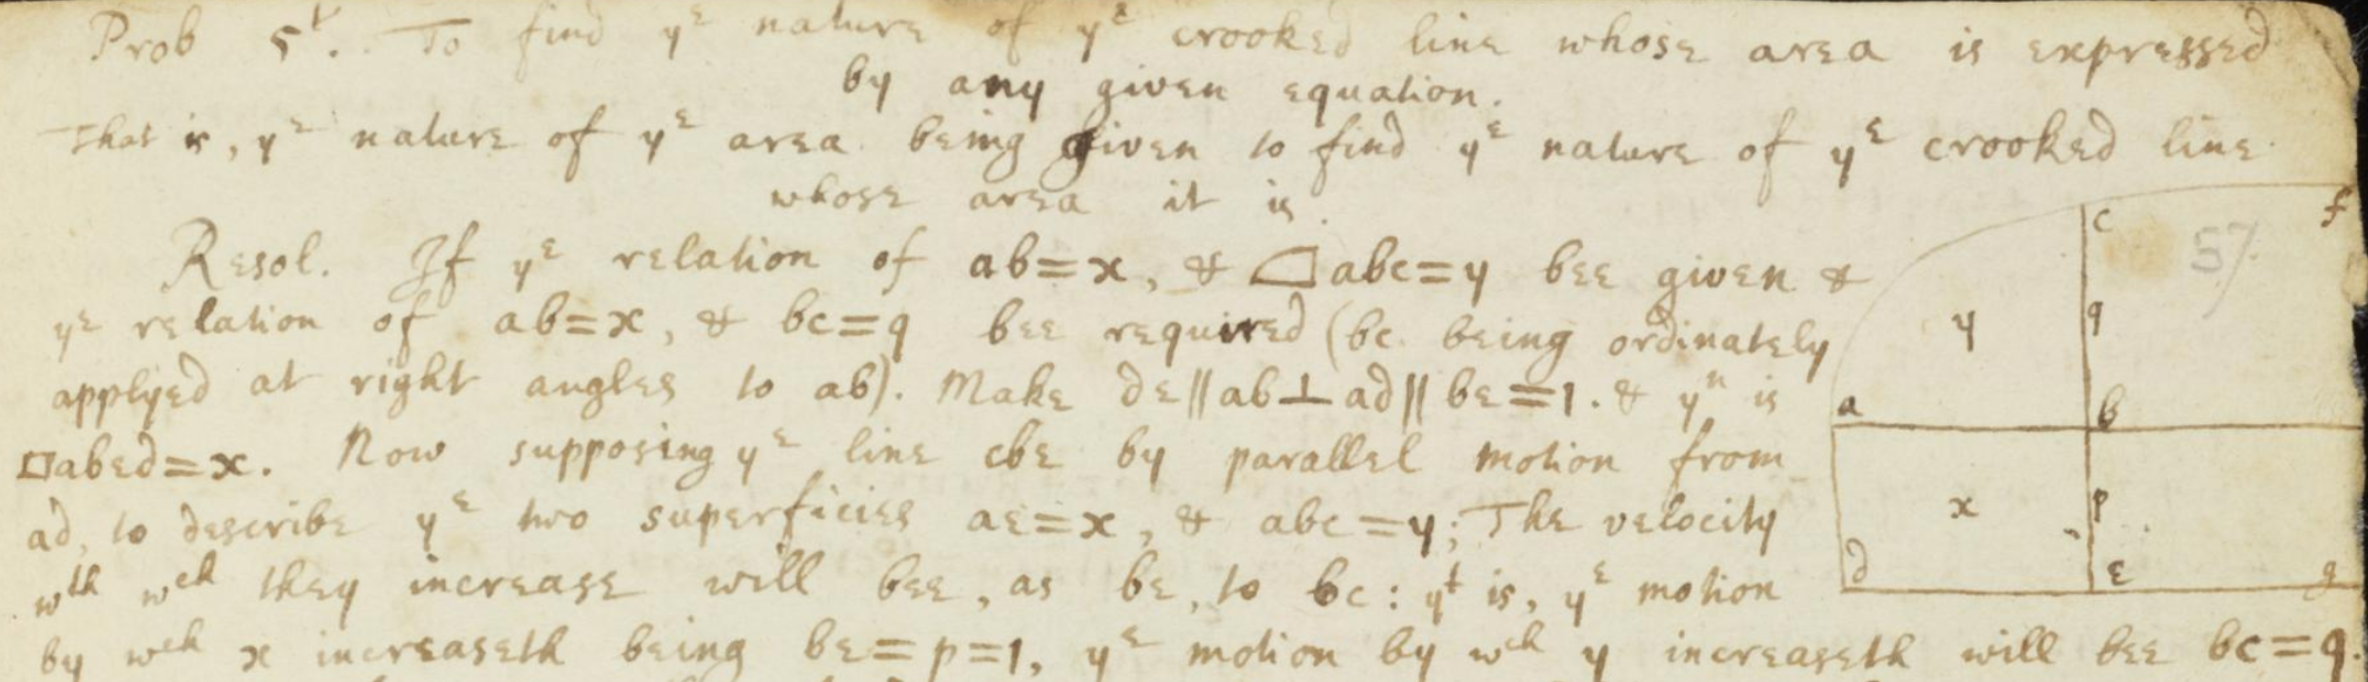
\includegraphics[width=500pt]{img/newton-october-1666-tract-ftc.png}
  \captionsetup{labelformat=empty,justification=centering}
  \caption[xxx]{Newton's October 1666 Tract on Fluxions.\\
    \emph{``...the motion by which y increaseth will bee $bc = q$.''}}
\end{figure}
\footnotetext{\url{https://cudl.lib.cam.ac.uk/view/MS-ADD-03958/109}}

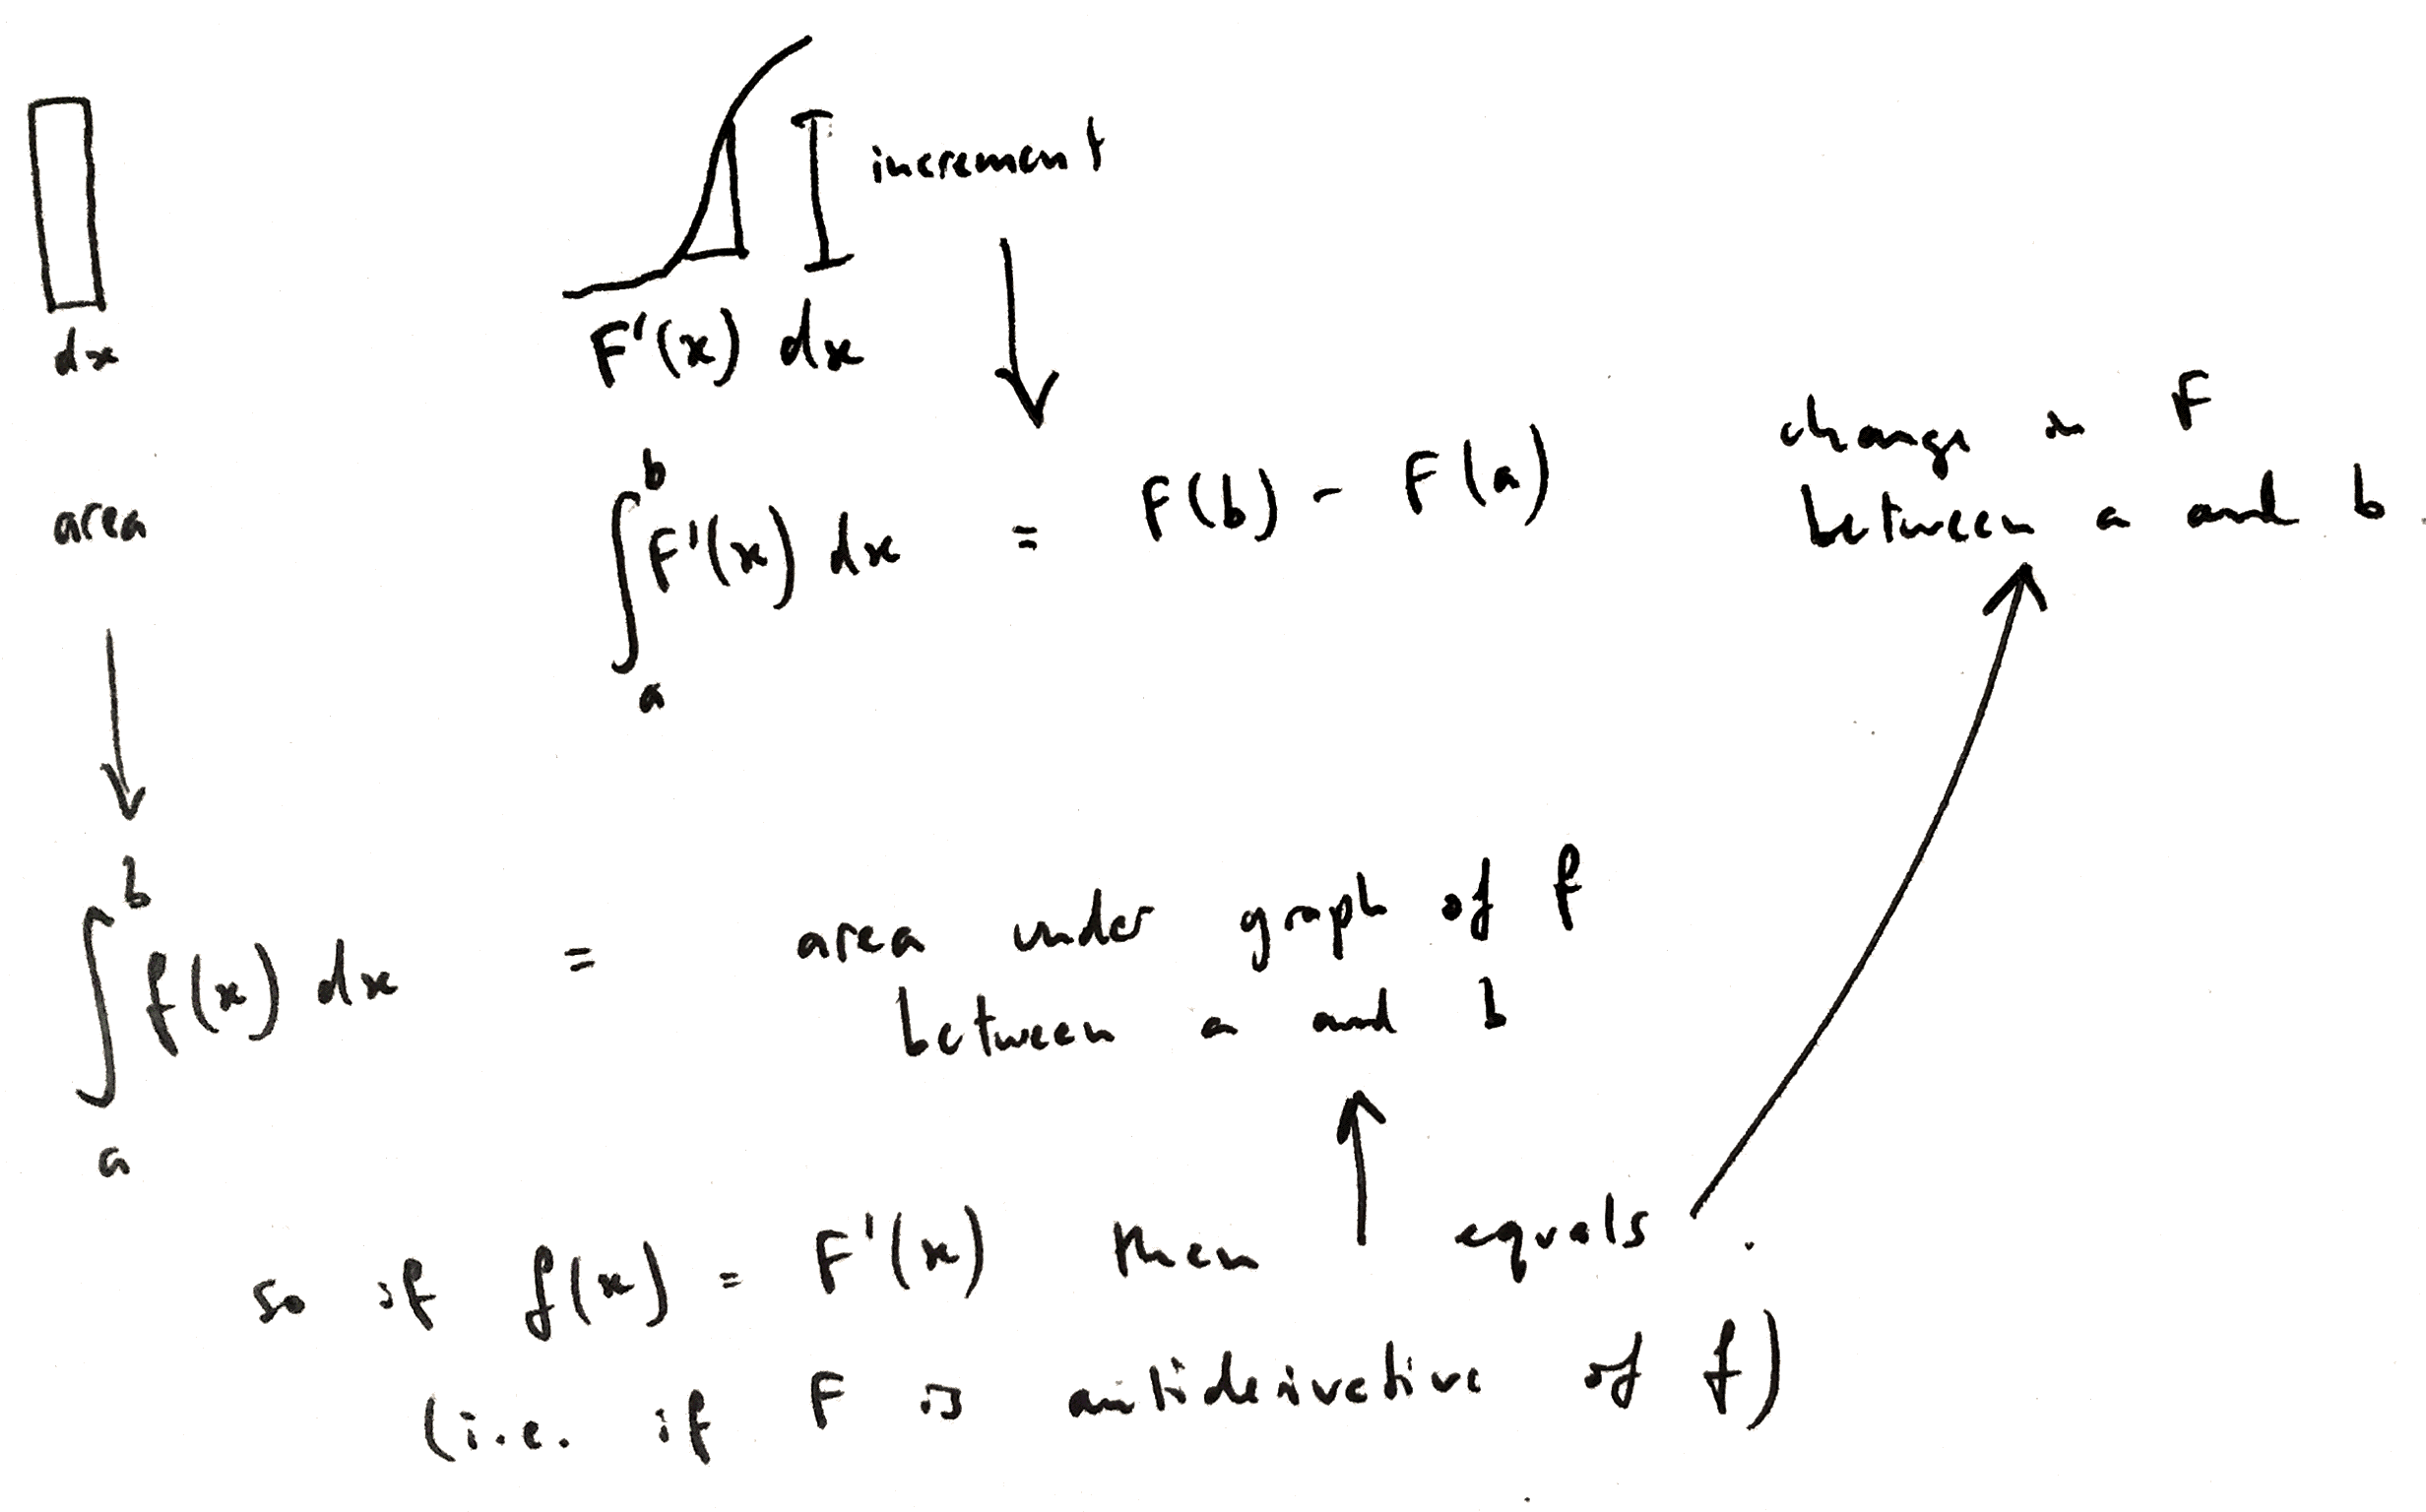
\includegraphics[width=300pt]{img/ftc.png}

Recall that the definition of $\int_a^b f(x) \dx$ is the area under the graph,
computed as the limit of approximating rectangles (Riemann sums).

Consider an ``accumulation function'', or ``area-so-far function'' $F$ defined
as
\begin{align*}
  F(x) = \int_0^x f(u) \d u.
\end{align*}

$F(x)$ is the amount that has accumulated when we are at point $x$ in the
input space.

The FTC comes in two parts. Part I states that the derivative of the
area-so-far function is the original function of interest:
\begin{align*}
  \ddx F(x) = f(x).
\end{align*}

Note that this is the first time we have connected integration with
differentiation: $F$ was defined as a definite integral (area-so-far); nothing
in its definition involved differentiation.

Part II states that the definite integral $\int_a^b f(x) \dx$ can be computed as
\begin{align*}
  \int_a^b f(x) \dx = F(b) - F(a).
\end{align*}
I think that this is obvious from the definition of $F$ as area-so-far, but the
point is that part I has shown us that $F$ might be obtainable as an
antiderivative of $f$ rather than via some explicit area calculation
(e.g. Riemann sums).

So how do we prove this? What exactly is it we need to prove anyway? We have a
definition for derivative, and we have a definition for area-so-far (limit of
Riemann sums). So, first, using the definition of derivative,
\begin{align*}
  \ddx F(x) := \lim_{h \to 0} \frac{F(x+h) - F(x)}{h}.
\end{align*}
In the numerator is the area above a horizontal section of width
$h$. Intuitively, this is approximately $hf(x)$, giving
\begin{align*}
  \ddx F(x) = \lim_{h \to 0} \frac{hf(x)}{h} = f(x),
\end{align*}
as desired. How to make this rigorous? Using the Riemann sums definition of area,
\begin{align*}
  \ddx F(x) &= \lim_{h \to 0} \frac{\lim_{N \to \infty} \sum_i^N \frac{h}{N} f\(x + \frac{ih}{N}\)}{h}\\
            &= \lim_{N \to \infty} \frac{1}{N} \sum_i^N \lim_{h \to 0} f\(x + \frac{ih}{N}\)\\
            &= \lim_{N \to \infty} \frac{1}{N} \sum_i^N f(x)\\
            &= f(x).
\end{align*}
But in fact real proofs use the Extreme Value Theorem. I am told that one error
in the above proof is that it is not valid to exchange the order of the two
limits.

TODO FTC -- moving away from thinking that an integral ``just has to end with
d-something''. Why does one seek the antiderivative of the part without the
d-something?

\subsubsection*{Examples}

In all the following examples, some quantity is
``accumulating''\footnote{``Accumulating'' can involve decreasing as well as
  increasing. For example if the particle starts moving back towards the
  origin, or if the vase is being filled with a tube and someone starts sucking
  on it rather than dispensing water.}.

\begin{enumerate}
\item $F(x)$ is the area under a graph to the left of $x$.\\
  $f(x)$ is the height of the graph at $x$.\\

\item $F(x)$ is the volume of a vase between the base and height $x$. \\
  $f(x)$ is the cross-sectional area at height $x$.\\

\item $F(r)$ is the area of a circle with radius $r$.\\
  $f(r)$ is the diameter of a circle with radius $r$.\\

\item $F(t)$ is the volume of water in a vase that is being filled, at time $t$.\\
  $f(t)$ is the rate of filling at time $t$.\\

\item $F(t)$ is the position of a moving particle at time $t$, relative to the origin.\\
  $f(t)$ is the velocity of the particle at time $t$.\\

\item $F(t)$ is the number of bacteria at time $t$.\\
  $f(t)$ is the rate at which new bacteria are produced at time $t$.
\end{enumerate}

\subsubsection*{Constant rate}
\begin{enumerate}
\item The height of the graph is constant at $h$ (a rectangle).\\
  The area to the left of $x$ is $hx$.\\

\item $F(x)$ is the volume of a vase between the base and height $x$. \\
  The cross-sectional area is constant at $a$ (a cylinder).\\
  $F(x) = ax$\\

\item $F(t)$ is the volume of water in a vase that is being filled, at time $t$.\\
  Water enters at a constant rate $v$ liters/sec.\\
  $F(t) = vt$\\

\item $F(t)$ is the displacement of a moving particle at time $t$, relative to the origin.\\
  The velocity of the particle is constant at $v$ m/sec.\\
  $F(t) = vt$.\\

\item $F(t)$ is the number of bacteria at time $t$.\\
  Bacteria are produced at a constant rate $v$ bacteria/sec.\\
  $F(t) = vt$.
\end{enumerate}

The amount-so-far can be computed manually:

\begin{enumerate}
\item If the rate of increase is constant at $v$, then the amount to the left
  of $x$ is simply $vx$.\\
\item If the rate of increase at time $t$ is $ct$ (proportional to $t$), then
  the amount-so-far graph is a triangle, so the amount to the left of $t$ is
  $\frac{1}{2}\cdot ct \cdot t = \frac{1}{2}ct^2$.\\
\item If the rate of increase at point $r$ is $2\pi r$ (the outer edge of a
  growing disc), then the amount-so-far graph is a triangle again, and the area
  of the disc is $\frac{1}{2}\cdot r \cdot 2\pi r = \pi r^2$.
\end{enumerate}

What about if the rate of increase is a more complex function? We can still
compute the area so far manually, as a limit of Riemann sums:

Compare
\begin{align*}
\int_0^2 (2 - x^2) \dx
  &= \lim_{N \to \infty}\sum_{i=1}^N \frac{2}{N}\(2 - \(\frac{2i}{N}\)^2\) \\
  &= \lim_{N \to \infty}\sum_{i=1}^N \frac{4}{N} - \frac{8i^2}{N^3} \\
  &= \lim_{N \to \infty}\(4  - \frac{8}{N^3}\sum_{i=1}^Ni^2 \)\\
  &= \lim_{N \to \infty}\(4  - \frac{8}{N^3}\frac{N(N+1)(2N+1)}{6} \)\\
  &= \lim_{N \to \infty}\(4  - 8\frac{(N+1)(2N+1)}{6N^2} \)\\
  &= \lim_{N \to \infty}\(4  - 8\frac{2 + 3N^{-1} + N^{-2}}{6} \)\\
  &= 4  - \frac{8}{3} = \frac{4}{3}\\
\end{align*}
with the solution using antiderivatives:
\begin{align*}
\int_0^2 (2 - x^2) \dx
  &= \left[2x - \frac{x^3}{3}\right]_0^2 \\
  &= 4 - \frac{8}{3} = \frac{4}{3}.
\end{align*}


\newpage
Let's fix a physical example for discussing FTC: a moving object. The key
quantity here is the distance from the starting point.

Next, before writing the equations that state the FTC, let's be clear about the
objects that are going to be involved in those equations. The most important
object is a function that gives the distance from the starting point as a
function of time.

More generally, this is an ``accumulation function'', or ``area-so-far
function''.

Now, let's introduce some notation. The notation $\int_3^4 f(t) \dt$ is
\textit{defined} to mean the area under the curve $f$, between $3$ and
$4$. It's really important to be clear here: the definition of
$\int_3^4 t^2 \dt$ is simply that it is the area under the $t^2$ curve between
those two points. (In particular, note that the definition does \textit{not}
involve $\frac{1}{3}t^3$).

Similarly, $\int_0^4 f(t) \dt$ is the area under the curve between 0 and 4. The
answer is a number. The answer doesn't involve $t$: $t$ is just a variable used
internally in that expression.

Now comes a slightly less obvious point: if the upper limit is not a fixed
number, but a variable, as in $\int_0^{x} f(t) \dt$, then that entire
expression represents a function of $x$: it takes in an $x$ value and outputs
the area under the curve, between 0 and $x$. We can give the new function a
name, $g$, and write the definition of $g$ as
\begin{align*}
  g(x) = \int_0^{x} f(t) \dt.
\end{align*}

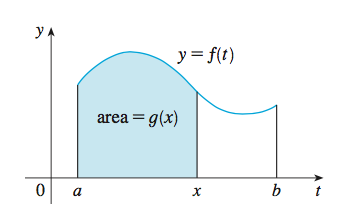
\includegraphics[width=200pt]{img/stewart-ftc-1.png}

Functions like $g$ are ``accumulation functions'', or ``area-so-far
functions'', because they tell you the area up to $x$, i.e. the area to the
left of $x$.

The FTC is usually split into two parts. The first part states\\
\begin{mdframed}
  At any point $x$, the rate of change of the area-so-far function at that
  point is the same as the height of the curve at that point.
\end{mdframed}

This is what Newton was saying when he wrote ``...the motion by which y
increaseth will bee $q$.'': in his diagram, $y$ is the area, and $q$ is the
height of the curve\footnote{He actually wrote ``$bc=q$''; $bc$ is a line in
  his diagram with length $q$.}.

\section{Differentiation basics}
\begin{theorem*}[Quotient rule]
  $\(\frac{f}{g}\)^\1 = \frac{gf' - fg'}{g^2}$
\end{theorem*}

\subsection{Derivatives of trigonometric functions}

\begin{claim*}
  $\tan' = \frac{1}{\cos^2} =: \sec^2$
\end{claim*}

\begin{proof}
  $\tan = \frac{\sin}{\cos}$, so by the quotient rule
  \begin{align*}
    \tan'
    = \frac{\cos^2 + \sin^2}{\cos^2}
    = \frac{1}{\cos^2}
    = \sec^2.
  \end{align*}
\end{proof}

\begin{claim*}
  What is the derivative of $\sin^\1$?
\end{claim*}

\begin{proof}
  \begin{align*}
    \frac{\d sin^\1 a}{\d a}
    = \frac{\d \theta}{\d \sin \theta}
    = \frac{1}{\cos \theta}
    = \frac{1}{\sqrt{1 - \sin^2 \theta }}
    = \frac{1}{\sqrt{1 - a^2}}
  \end{align*}
\end{proof}


\begin{claim*}
  What is the derivative of $\tan^\1$?
\end{claim*}

\begin{proof}
  \begin{align*}
    \frac{\d \tan^\1(a)}{\d a}
    = \frac{\d \theta}{\d \tan(\theta)}
    = \cos^2(\theta)
    = \cos^2(\tan^\1 a)
  \end{align*}
  Note that a right-angle triangle with angle $\tan^\1 a$ has opposite length $a$ relative to
  adjacent length 1. Therefore $\cos(\tan^\1 a) = \frac{1}{\sqrt{1 + a^2}}$.

  Therefore the derivative of $\tan^\1(a)$ is $\frac{1}{1 + a^2}$.
\end{proof}


\newpage
\section{Berkeley Math 53 (Frenkel)}
\subsection{Curves and surfaces}

A function is a rule associating input values from one set with output values
from another; a function is a set of (input, output) pairs in which each input
value occurs at most once.

A curve in $d$ dimensions is a set of $d$-dimensional points that form a
``connected'' 1-dimensional object.

A surface is a similar concept to a curve, but is 2-dimensional.

The dimensionality of an object is equal to the dimensionality of the ambient
space, minus the number of independent equations.

\subsection{Specifying a curve or surface}

\textbf{Cartesian equation:} A curve can be specified as the set of points
satisfying some condition (e.g. $x^2 + y^2 = R^2$) or by specifying that one
dimension records the value of a function whose inputs are the other
dimensions ($z = 3 + 1.5(x-1) - 2.7(y-2)$).

\textbf{Graph:} Let $f$ be $\R \to \R$. The graph of $f$ is the set of points
$(x,y)$ satisfying $y = f(x)$. This defines a curve in 2D (which never ``turns
back on itself''; the tangent line to the curve is never vertical.)

A curve in 3D would require two equations (to reduce the dimensionality of the
ambient space to that of the object being specified; i.e. the intersection of
two surfaces). In practice, curves in 3D are usually specified in parametric
form.

\textbf{Parametric form:} For a curve in 2D, suppose the x-coordinate is given
by $f(t)$ and the y-coordinate by $g(t)$. Then the curve is the set of points
$\big(f(t), g(t)\big)$ for some range of the parameter $t$. E.g. a line
represented in parametric form using vector notation:
$\vec r = \vec r_0 + \vec v t$. (A surface would require 2 parameters, so they
are often specified using Cartesian equations.)


\subsection{Area under a curve}

What is the area $A$ under the curve from $t=a$ to $t=b$? It's just
$\int_\alpha^\beta y \dx$ as usual\footnote{$(\alpha, \beta) = (f(a), f(b))$},
but how do we express this as an integral with respect to $t$?

Well, $y = g(t)$; what about $\dx$? $x = f(t)$ (displacement), therefore
$\dx = \dt f'(t)$ (velocity $\times$ time; local linear approximation). So, the
area under the curve bounded by start and end $t$-values is
$A = \int_a^b g(t) f'(t) \dt$.

Thus, if the x-coordinate is increasing rapidly with $t$, then the area is
larger.

\subsection{Length of a curve}

The length of a curve is $L = \int \sqrt{\dx^2 + \dy^2}$, over some interval.

This can be expressed as an integral with respect to $x$ (non-parametric form):
$L = \int_\alpha^\beta \sqrt{1 + (\frac{\dy}{\dx})^2} \dx$.

Or it can be expressed as an integral over an interval of $t$ values (parametric form):
$L = \int_a^b \sqrt{ (\frac{\dx}{\dt})^2 + (\frac{\dy}{\dt})^2} \dt$

\subsection{Area and volume of revolution of a curve}
Suppose a curve is revolved around the $x$-axis.

\textbf{Volume}\\
This is computed as a sum of discs with width $\dx$:
\begin{align*}
  V = \int_{x=\alpha}^{x=\beta} \pi y^2 \dx.
\end{align*}
\textbf{Area}\\
This is computed as a sum of strips (using the hypotenuse rather than the rectangular strips used for the volume\footnote{Why exactly do we
  construct these strips using the hypotenuse, whereas when approximating the
  area under a graph we construct rectangles $y\dx$? See \\
  \url{https://math.stackexchange.com/questions/1691147/why-is-surface-area-not-simply-2-pi-int-ab-y-dx-instead-of-2-pi-in}\\
  \url{https://math.stackexchange.com/questions/1074986/surface-area-of-a-solid-of-revolution-why-does-not-int-ba-2-pi-fx}\\
  \url{https://math.stackexchange.com/questions/12906/is-value-of-pi-4}}):
\begin{align*}
  A = \int_{x=\alpha}^{x=\beta}  2\pi y \sqrt{\dx^2 + \dy^2}
\end{align*}


\subsection{Polar coordinates}

E.g. the curve $r = \cos(\theta)$ is a circle of radius 1 centered at
$(x, y) = (\frac{1}{2}, 0)$. (?)

\subsection*{Area of a sector bounded by a curve}

What's the area of the sector bounded by the two rays and a curve, between
$\theta=a$ and $\theta=b$?

Note that the area of a sector of $\phi$ radians of a circle is
$\pi r^2 \times \frac{\phi}{2\pi} = \frac{1}{2}\phi r^2$.

We're considering a curve defined by $r = f(\theta)$. We divide it up into many
sectors each with angle $\dtheta$. The area is
$\int_a^b \frac{1}{2}f(\theta)^2\dtheta$.

\subsection{Surfaces}

\subsection*{Planes}
Given a normal vector $\vec n = \cveccc{d}{e}{f}$, and a point in the plane
$P = \cveccc{x_0}{y_0}{z_0}$, an equation specifying the plane is

\begin{align*}
  d(x - x_0) + e(y - y_0) + f(z - z_0) = 0 \\
  dx + ey + fz = C.
\end{align*}

So the normal vector can be read off from the equation.

Similarly the general equation of a line in 2D is

\begin{align*}
  d(x - x_0) + e(y - y_0) = 0,
\end{align*}

(TODO: explain this and other content towards end of L11)

so $\cvecc{d}{e}$ is a normal vector to the line.


\subsection*{Quadric surfaces}
Ellipsoids, hyperboloids, paraboloids. Also cylinders (one variable not
specified, e.g. $x^2 + y^2 = 1$), and cones (e.g. $z^2 = x^2 + y^2$).

\subsection{Tangent spaces}

\subsection*{Tangent lines}
E.g. a tangent vector is given by differentiating the parametric equation for a
curve, giving an equation for the tangent line:

\begin{align*}
  \vec r = \vec r_0 + \cveccc{x'(t_0)}{y'(t_0)}{z'(t_0)}s = \vec r_0 + \vec v' s.
\end{align*}

\subsection*{Tangent planes}

\begin{align*}
  (z - z_o) = (x - x_0)f_x(x_0, y_0) + (y - y_0)f_y(x_0, y_0)
\end{align*}

And what's the normal vector to that tangent plane? It's
$\cveccc{f_x(x_0, y_0)}{f_y(x_0, y_0)}{-1}$.


\subsection{Limits (L8)}

$\frac{x^2}{x^2 + y^2}$ has no limit at $(0, 0)$.
Easy to prove by exhibiting paths with different limits: e.g. along x-axis vs. y-axis.
Lack of limit related to degree of numerator and denominator being same.

But $\frac{2x^3}{x^2 + y^2}$ does have a limit at $(0, 0)$.

Proof: consider a disk of radius $r$. For points in this disk, $x^2 + y^2 \leq r^2$ and so $x \leq r$.
Now

\begin{align*}
  \left|\frac{2x^3}{x^2 + y^2}\right| = 2|x|\left|\frac{x^2}{x^2 + y^2}\right| \leq 2r,
\end{align*}

so for any desired closeness to the limiting value 0, we can find an $r$ that will do it.

\subsection{Partial derivatives (L8)}

Clairot's theorem: equality of mixed partials under certain continuity
conditions.

\begin{quote}
  ``Same commutative structure as multiplication''; all that matters
  is how many times you have differentiated w.r.t. $x$, and to $y$;
  ``differentiation is in a sense opposite to multiplication''.
\end{quote}

\subsection{Differentials (L8)}

\begin{quote}
  ``The differential is the function whose graph the tangent line (plane) is,
  but with the coordinate axes shifted to the point at which it is being
  evaluated.''
\end{quote}

A differential, defined at a particular point in the input space, is the
function describing the linear approximation at that point: it maps a
displacement in the input space to a displacement in the output space.

It's the function whose graph is the tangent space at that point, in a
coordinate space shifted to have its origin at that point. So in 1D, if
$z = f(x)$, then the differential at $x_0$ is

\begin{align*}
  \dz(x) = (x - x_0)f'(x_0).
\end{align*}


Not to be confused with $\Delta f$ --- the increment in the \textit{actual
  function} value --- whereas the differential refers to the increment in the
linear approximation.


\subsection{Directional derivatives (L11)}

TODO Note: Defining directional derivative as being a function of a \textit{unit} vector is
controversial; see
e.g. \url{https://math.stackexchange.com/questions/2291302/why-isnt-the-directional-derivative-generally-scaled-down-to-the-unit-vector}
The majority view is, contra Stewart, that the directional derivative should be defined as a
function of a vector of any magnitude. The interpretation of that is that it gives the rate of
change of the function as you move past the point with velocity given by the vector $u$. One
motivation is that this makes it linear in $u$: $dd(u + v) = dd(u) + dd(v)$ etc.

\theorem{
  The directional derivative of $f(x, y)$ in the direction of a unit
  vector $u = \cvecc{a}{b}$ is
  \begin{align*}
    D_u f = a\partiald{f}{x} + b\partiald{f}{y} = \nabla f \cdot \vec u.
  \end{align*}
}

\proof{ Since $u$ is unit length, $\cvecc{ha}{hb}$ is a displacement of length
  $h$ in the direction of $u$. Then\footnote{The proof in the lecture and in
    Stewart is slightly different, involving defining these quantities as
    functions of $h$ and considering the derivative w.r.t. $h$.}
  \begin{align*}
    D_u f(x_0, y_0)
    :=& \lim_{h \to 0} \frac{f(x_0 + ha, y_0 + hb) - f(x_0, y_0)}{h} \\
    =& \lim_{h \to 0} \frac{f(x_0, y_0) + ha\partiald{f}{x}(x_0, y_0) + hb\partiald{f}{y}(x_0, y_0) - f(x_0, y_0)}{h} \\
    =& a\partiald{f}{x}(x_0, y_0) + b\partiald{f}{y}(x_0, y_0) \qed
  \end{align*}

}

\subsection{Gradient}
$\nabla f(x_0, y_0)$ is normal to the level curve that cuts $f$ at $z = z_0$.

Recall that $\cveccc{f_x(x_0,y_0)}{f_y(x_0,y_0)}{-1}$ is a normal vector to the
tangent plane at $(x_0,y_0)$.


\section{Linear and quadratic approximations to a function}
\footnote{
  \href{https://www.khanacademy.org/math/multivariable-calculus/applications-of-multivariable-derivatives/optimizing-multivariable-functions/a/reasoning-behind-the-second-partial-derivative-test}{khanacademy - Grant Sanderson - second partial derivative test}
}




We construct first- and second-order approximations to a differentiable
function $f: \R^2 \rightarrow \R$. The approximation is made at some point
$(x_0, y_0) = \vec x_0 \in \R^2$; we demand that the value of the approximation, and the
first and second derivatives, match those of $f$ exactly at that point.

\subsection{Linear approximation to a function $f(x, y)$ near $(x_0, y_0)$:}

\begin{align*}
L(x, y) &=
~
f(x_0, y_0) ~+
(x - x_0)f_x(x_0,y_0) +
(y - y_0)f_y(x_0,y_0)
\\\\
&= f(\vec x) + (\vec x - \vec x_0) \cdot \nabla_f(\vec x_0)
\end{align*}

Note that, at $(x_0, y_0)$, the first partial derivatives of $L$ are equal to
those of $f$, as they must be. (In fact, we could say that the coefficients are
determined by this requirement; see the quadratic case below. But the linear
case is obvious without ``deriving'' the coefficients.)


\subsection{Quadratic approximation to a function $f(x, y)$ near $(x_0, y_0)$:}

The $j$-th component of the gradient of $q(\x) = \x^\T A \x$ is
$\partiald{q}{x_j} = 2\sum_k A_{jk}x_k$, so
\begin{align*}
  \nabla ~\x^\T \vec A \x = 2\vec A \x.
\end{align*}

\begin{align*}
Q(x, y) &=
f(\vec x_0) + (x - x_0)f_x(\vec x_0) +
(y - y_0)f_y(\vec x_0) ~+ \\
&~~~~~~~\frac{1}{2} f_{xx}(\vec x_0)(x - x_0)^2 +
f_{xy}(\vec x_0)(x - x_0)(y - y_0) +
\frac{1}{2} f_{yy}(\vec x_0)(y - y_0)^2 \\\\
&= f(\vec x_0) +
(\vec x - \vec x_0) \cdot \nabla f(\vec x_0) +
\frac{1}{2}(\vec x - \vec x_0)^\T \nabla^2 f(\vec x_0)(\vec x - \vec x_0),
\end{align*}
where $\nabla^2 f(\vec x_0)$ is the Hessian matrix $\mat{f_{xx}}{f_{xy}}
{f_{yx}}{f_{yy}}$ evaluated at $\vec x_0$.

\subsection{Second partial derivative test and positive definiteness of Hessian}

The second partial derivative test for a function of two variables states that
we examine the determinant of the Hessian evaluated at the critical point:
$$
D = \det \nabla^2 f(\vec x_0) = f_{xx}(\vec x_0)f_{yy}(\vec x_0) - f_{xy}(\vec x_0)^2.
$$

Notice that $D \geq 0$ implies that the sign of $f_{xx}$ and $f_{yy}$ agree
(because we're subtracting the square of the mixed partial $f_{xy}$, i.e. a
positive number).

\begin{tabular}{ l l l l l }
  $D$    & roots          & $f_{xx}$ &  & Hessian \\
  \hline
  $+$    & no real roots  & $+$     & minimum        & positive definite \\
  $+$    & no real roots  & $-$     & maximum        & negative definite \\
  $0$    & one real root  & $+$     & minimum        & positive semidefinite \\
  $0$    & one real root  & $-$     & maximum        & negative semidefinite \\
  $-$    & two real roots & n/a     & saddle point   & - \\
\end{tabular}

\subsubsection*{Explanation}
At a critical point $\vec x_0$, the gradient is zero and the quadratic approximation is therefore
$$
Q(x, y) = f(\vec x_0) + \frac{1}{2}(\vec x - \vec x_0)^\T \nabla^2 f(\vec x_0)(\vec x - \vec x_0).
$$
So if this is a minimum (concave-up paraboloid) then this quadratic form is
positive for all $\vec x \neq \vec x_0$ (and if it's a maximum then it's
negative for all $\vec x \neq \vec x_0$).

Basically the argument is that, instead of analyzing the function $f$ itself,
we analyze its quadratic approximation at the critical point. So the question
comes down to: how do we determine whether a quadratic form is always positive,
always negative, or takes positive and negative values?

To answer that, consider a generic quadratic form $ax^2 + 2bxy + cy^2$. Let $y$
be constant at $y_0$; then we have a quadratic in $x$, the roots of which are
\begin{align*}
  x
  = \frac{-2by_0 \pm \sqrt{4b^2y_0^2 - 4acy_0^2}}{2a}
  = y_0\frac{-b \pm \sqrt{b^2 - ac}}{a}.
\end{align*}
So, whether this is a saddle point or a minimum/maximum depends on whether the
quadratic form has real roots. If there are no real roots, then whether it's a
minimum or a maximum depends on the sign of $f_{xx}$ (this sign will be the
same as that of $f_{yy}$ in the no real roots case).

\subsection{Derivation of quadratic approximation coefficients}
\begin{align*}
Q(x, y) =
&f(\vec x_0) + (x - x_0)f_x(\vec x_0) +
(y - y_0)f_y(\vec x_0) ~+ \\
&a(x - x_0)^2 +
b(x - x_0)(y - y_0) +
c(y - y_0)^2
\end{align*}

What are the coefficients $a,b,c$? They are determined by the requirement that
the second partial derivatives are identical at the point of approximation
$\vec x_0$.

First look at the first partial derivatives:

\begin{align*}
  Q_x &= f_x(\vec x_0) + 2a(x - x_0) + b(y - y_0)\\
  Q_y &= f_y(\vec x_0) + b(x - x_0) + 2c(y - y_0)\\
\end{align*}
so the quadratic approximation is an exact first-order approximation at $\vec x_0$, as required:
\begin{align*}
  Q_x(\vec x_0) &= f_x(\vec x_0) \\
  Q_y(\vec x_0) &= f_y(\vec x_0),
\end{align*}

Now look at the second derivatives:
\begin{align*}
  Q_{xx} &= 0 + 2a + 0 \\
  Q_{xy} &= 0 + 0 + b \\
  Q_{yx} &= 0 + b + 0 \\
  Q_{yy} &= 0 + 0 + 2c \\
\end{align*}
Since we require that these match those of $f$ exactly at $\vec x_0$, we have
\begin{align*}
  a &= \frac{1}{2} f_{xx}(\vec x_0) \\
  b &= f_{xy}(\vec x_0) = f_{yx}(\vec x_0) \\
  c &= \frac{1}{2} f_{yy}(\vec x_0),
\end{align*}
so the quadratic approximation is
\begin{align*}
Q(x, y) =
&f(\vec x_0) + (x - x_0)f_x(\vec x_0) +
(y - y_0)f_y(\vec x_0) ~+ \\
&\frac{1}{2} f_{xx}(\vec x_0)(x - x_0)^2 +
f_{xy}(\vec x_0)(x - x_0)(y - y_0) +
\frac{1}{2} f_{yy}(\vec x_0)(y - y_0)^2
\end{align*}

\section{Oxford M5 Multivariable calculus}

\subsection{Integrals in two dimensions}

\begin{example*}[5]

\end{example*}

\begin{proof}
  \begin{align*}
    \int \int_R (x + y^2) \dx\dy
    &= \int_1^3 \int_0^2 (x + y^2) \dx\dy\\
    &= \int_1^3 \Big(\frac{x^2}{2} + xy^2\Big)\Big|_{x=0}^{x=2} \dy\\
    &= \int_1^3 2 + 2y^2 \dy\\
    &= 2y + \frac{2y^3}{3} \Big|_1^3\\
    &= 6 + 18 - 2 - \frac{2}{3}\\
    &= \frac{64}{3}
  \end{align*}
\end{proof}


\begin{example*}[6]
  Let $R$ be the unit square. Determine $\int\int_R y\cos^2(\pi xy) dA$.
\end{example*}

\red{TODO}

\begin{proof}
  \begin{align*}
    \int\int_R y\cos^2(\pi xy) dA
    &= \int_0^1\int_0^1 y\cos^2(\pi xy) \dx\dy\\
    &=
    &=
  \end{align*}
\end{proof}

\begin{mdframed}
  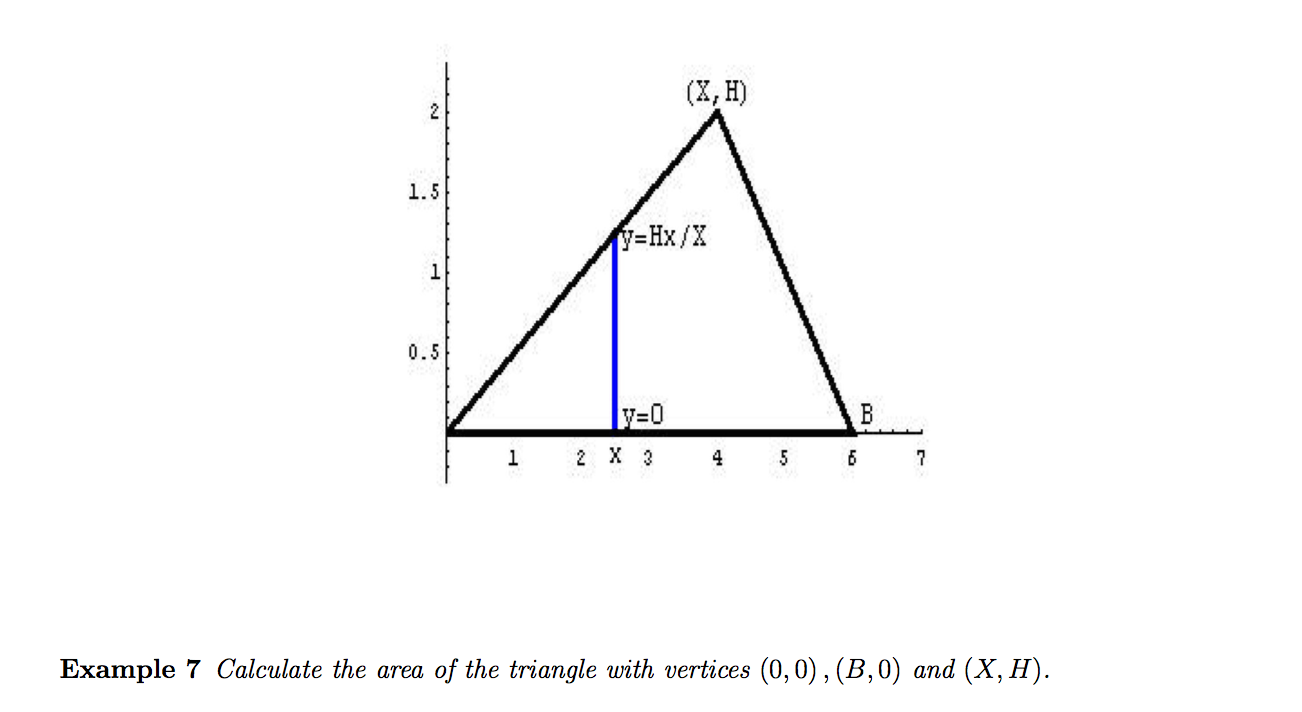
\includegraphics[width=400pt]{img/oxford-prelims-M5-multivariable-calc-ex-7.png}
\end{mdframed}


\begin{proof}(I. sum of two one-dimensional integrals)
\end{proof}

\begin{proof}(II. sum of two integrals over area)\\
  The triangle is composed of a piecewise linear function:
  \begin{align*}
    \text{height}(x) =
    \begin{cases}
      x\frac{H}{X}, ~~~~~~~~~~~~~~~~~~     0 \leq x \leq X\\
      (x - B)\frac{H}{(X - B)}, ~~~~~~~ X < x \leq B.
    \end{cases}
  \end{align*}

  \begin{align*}
    \text{area} &= \int\int_R dA\\
                &= \int_0^X \int_0^{xH/X} \dy \dx + \int_X^B\int_0^{(x - B)\frac{H}{(X - B)}}\dy\dx\\
                &= \int_0^X xH/X \dx + \int_X^B (x - B)\frac{H}{(X - B)} \dx\\
                &= \frac{H}{X}\int_0^X x \dx + \frac{H}{(X - B)}\int_X^B (x - B) \dx\\
                &= \frac{HX^2}{2X} + \frac{H}{(X - B)}\Big[\frac{(x - B)^2}{2}\Big]_X^B\\
                &= \frac{HX}{2} - \frac{H}{(X - B)}\frac{(X - B)^2}{2}\\
                &= \frac{HX}{2} - \frac{H(X - B)}{2}\\
                &= \frac{BH}{2}
  \end{align*}
\end{proof}


\newpage
\subsection{Change of variables and Jacobians}
Let $R, S \subset \R$ and $u:R \to S$.

Define $\psi: R \to \R$ and $\Psi: S \to \R$, such that $\Psi(f(x)) = \psi(x)$ for all $x \in R$.

One definition of the integral is to divide $R$ into segments of length $\delta x$, let $\psi_i$ be
the value of $\psi$ at the start of the $i$-th segment, and define
\begin{align*}
  \int_{x \in R} \psi(x) \dx = \lim_{\delta x \to 0} \sum_i \psi_i\delta x.
\end{align*}

Now let $u'_i$ be the value of the derivative at the start of the $i$-th line segment.

Then the length of the $i$-th segment of $S$ is $u'_i ~\delta x$.

Therefore the integral over $S$ is
\begin{align*}
  \int_{u \in S} \Psi(u) \du &= \lim_{\delta x \to 0} \sum_i \psi_iu'_i~\delta x\\
                            &= \int_{x \in R} \psi(x)\frac{\du}{\dx}\dx.
\end{align*}

\newpage
\begin{theorem*}[Integration by substitution]~\\
  Let $u = h(x)$. Then
  \begin{align*}
    \int g(h(x))h'(x) \dx = \int g(u) \du.
  \end{align*}
\end{theorem*}

\begin{proof}
  Let $G' = g$, i.e. $G$ is an antiderivative of $g$.

  Recall the chain rule:
  \begin{align*}
    (G \circ h)' = G' h'
  \end{align*}
  Integrating both sides with respect to $x$ gives
  \begin{align*}
    G \circ h + C = \int G' h' \dx = \int g h' \dx.
  \end{align*}
  Let $u = h(x)$. Then
  \begin{align*}
    G(u) + C &= \int g(u) \du
              = \int \frac{\dG}{\dh} \frac{\du}{\dx} \dx.
  \end{align*}
\end{proof}

\begin{proof}
  Let $G' = g$, i.e. $G$ is an antiderivative of $g$.

  Recall the chain rule:
  \begin{align*}
    \ddx G(h(x)) = \frac{\dG}{\dh} \frac{\dh}{\dx}.
  \end{align*}
  Integrating both sides with respect to $x$ gives
  \begin{align*}
    G(h(x)) + C = \int \frac{\dG}{\dh} \frac{\dh}{\dx} \dx.
  \end{align*}
  Let $u = h(x)$. Then
  \begin{align*}
    G(u) + C &= \int g(u) \du
              = \int \frac{\dG}{\dh} \frac{\du}{\dx} \dx.
  \end{align*}
\end{proof}

\begin{definition*}[Jacobian]
  Let $f:\R^2 \to \R^2$ be given by $f(x, y) := (u(x, y), v(x, y))$.

  The Jacobian of $f$ is
  $
  \frac{\partial(u, v)}{\partial(x, y)} =
  \det \matMMxNN{\frac{\partial u}{\partial x}} {\frac{\partial u}{\partial y}}
  {\frac{\partial v}{\partial x}} {\frac{\partial v}{\partial y}}
  = \det \matMMxNN{u_x}{u_y}
  {v_x}{v_y}.
  $

  It is defined analogously in 3D.
\end{definition*}

\begin{theorem}\label{stretch-factor-is-jacobian}
  The Jacobian of a map is the factor by which the map stretches space locally.
\end{theorem}

\begin{proof}(Sketch)\\
  Let $f: \R^2\to\R^2$ be a differentiable function given by
  $(x,y) \mapsto \Big(u(x,y), v(x,y)\Big)$.

  Consider a small rectangular area with bottom-left corner $(x, y)$ and top-right corner
  $(x + \delta x, y + \delta y)$.

  Let $u_x, u_y, v_x, v_y$ be the partial derivatives evaluated at $(x, y)$.

  The linear approximation to $f$ at $(x, y)$ is
  \begin{align*}
    f(x, y) \approx  f(x, y) +
    \cvec
    {u_x\delta x + u_y\delta y}
    {v_x\delta x + v_y\delta y}
  \end{align*}

  So the bottom-right and top-left corners are mapped as follows:
  \begin{align*}
    \text{bottom right:~~~}&
                             (x, y) \mapsto f(x, y) +
                             \cvec
                             {u_x\delta x}
                             {v_x\delta x}
    \\
    \text{top left:~~~}&
                         (x, y) \mapsto f(x, y) +
                         \cvec
                         {u_y\delta y}
                         {v_y\delta y}
  \end{align*}

  Thus the image of the original rectangular area is a parallelogram spanned by the vectors
  $\delta x\cvec{u_x}{v_x}$ and $\delta y\cvec{u_y}{v_y}$. The area of this parallelogram is given by
  the cross product:
  \begin{align*}
    \text{area}
    = \Bigg|\delta x\cvec{u_x}{v_x} \times
    \delta y\cvec{u_y}{v_y}\Bigg|
    = |(u_xv_y - u_yv_x)\mathbf{k}|\delta x \delta y
    = \det \matMMxNN{u_x}{u_y}
    {v_x}{v_y} \delta x \delta y.
  \end{align*}


\end{proof}


\begin{example*}
  Let $x = r\cos\theta$ and $y = r\sin\theta$, where $r$ and $\theta$ are polar co-ordinates. Then
  \begin{align*}
    \frac{\partial(x, y)}{\partial(r, \theta)}
    &= \det \matMMxNN{\cos\theta}{-r\sin\theta}
                     {\sin\theta}{r\cos\theta}\\
    &= r(\cos^2\theta + \sin^2\theta)\\
    &= r.
  \end{align*}
\end{example*}

\begin{example*}
  In reverse, $r(x,y) = \sqrt{x^2 + y^2}$ and $\theta(x,y) = \tan^\1(y/x)$.

  Note that $\partiald{\theta}{x} = \frac{1}{1 + \frac{y^2}{x^2}}\frac{-y}{x^2} = \frac{-y}{x^2 + y^2}$,
  and $\partiald{\theta}{y} = \frac{1}{1 + \frac{y^2}{x^2}}\frac{1}{x} = \frac{x}{x^2 + y^2}$.

  So
  \begin{align*}
    \frac{\partial(r, \theta)}{\partial(x, y)}
    &= \det \matMMxNN{\frac{x}{\sqrt{x^2 + y^2}}}{\frac{y}{\sqrt{x^2 + y^2}}}
                     {\frac{-y}{x^2 + y^2}      }{\frac{x}{x^2 + y^2}}\\
    &= \frac{x^2 + y^2}{(x^2+y^2)^{2/3}}\\
    &= \frac{1}{r}.
  \end{align*}
\end{example*}

\begin{theorem*}~\\
  Let:
  \begin{enumerate}
  \item $R, S \seq \R^2$
  \item $f:R \to S$ given by $f(x,y) = (u(x,y), v(x,y))$
  \item $\psi(x, y) = \Psi(u, v) = \Psi(u(x,y), v(x, y))$.
  \end{enumerate}
  Then
  \begin{align*}
    \int\int_{(x,y) \in R} \psi(x,y)\dx \dy
    &= \int\int_{(u, v) \in S} \Psi(u, v)\Big|\frac{\partial(x, y)}{\partial(u, v)}\Big|\du \d v\\
    \int\int_{(u,v) \in S} \Psi(u,v)\du \d v
    &= \int\int_{(x, y) \in R} \psi(x, y)\Big|\frac{\partial(u, v)}{\partial(x, y)}\Big|\dx \dy.
  \end{align*}
\end{theorem*}

\begin{mdframed}
  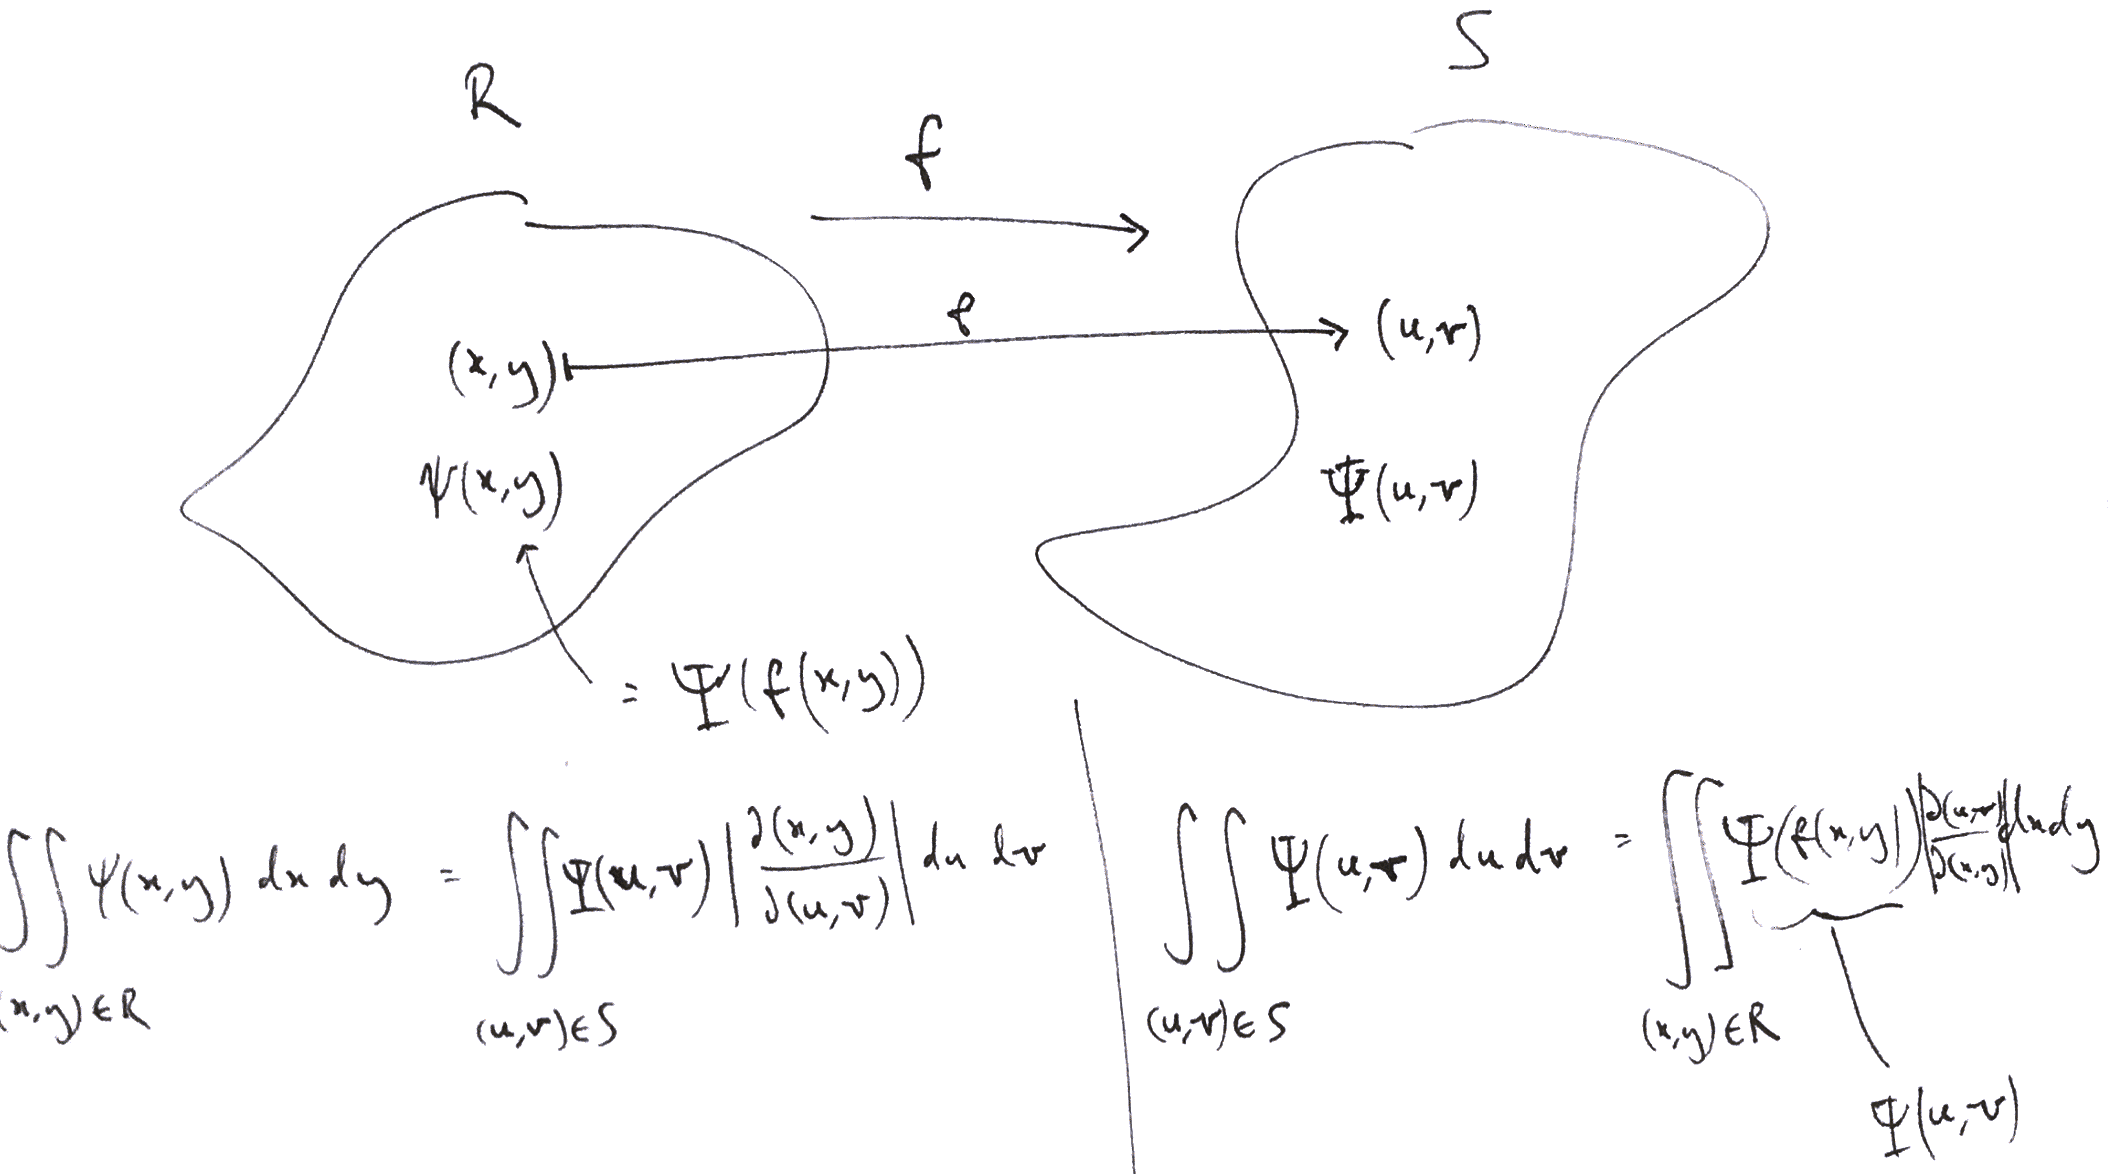
\includegraphics[width=300pt]{img/calculus-jacobian-2D-map.png}
\end{mdframed}

\begin{intuition*}
  If $f$ stretches space locally, then a local value $\psi(x,y)$ over $R$ contributes more when
  accumulating $\Psi$ values over $S$.
\end{intuition*}

\begin{proof}(Sketch)\\
  Divide $R$ into $N$ small squares.

  Let $u_x, u_u, v_x, v_y$ be the partial derivatives evaluated at the center of the $i$-th square.

  Note from theorem (\ref{stretch-factor-is-jacobian}) above that the image of the $i$-th square is
  a parallelogram with area $\vmatMMxNN {u_x}{u_y} {v_x}{v_y} \delta x \delta y$.

  An approximation for the integral over $S$ is
  \begin{align*}
    \int\int_{(u,v) \in S} \Psi(u,v)\du \d v
    &\approx \sum_i \Psi_i \text{Area(Parallelogram$_i$)}\\
    &= \sum_i \psi_i \vmatMMxNN
      {u_x}{u_y}
      {v_x}{v_y} \delta x \delta y,
  \end{align*}
  which on taking the limit $N \to \infty$ gives
  \begin{align*}
    \int\int_{(u,v) \in S} \Psi(u,v)\du \d v =
    \int\int_{(x,y) \in R} \psi(x,y) \Big|\frac{\partial(u, v)}{\partial(x, y)}\Big| \dx \dy.
  \end{align*}
\end{proof}

\newpage
\begin{mdframed}
  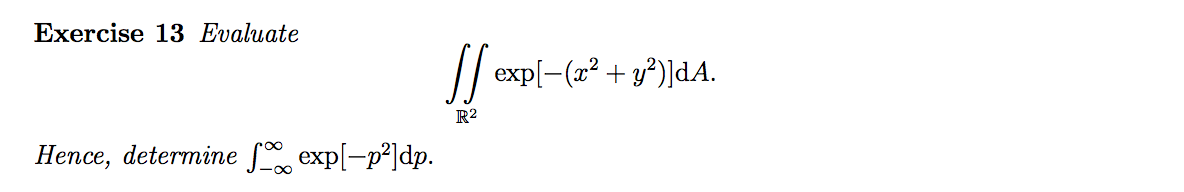
\includegraphics[width=400pt]{img/oxford-prelims-M5-multivariable-calc-ex-13.png}
\end{mdframed}

First of all, note that $\int_{-\infty}^{\infty}e^{-x}\dx$ does not converge, and that it is not
obvious how to calculate $\int_{-\infty}^{\infty}e^{-x^2}\dx$.

\begin{proof}
  Let $f(x,y) = (r, \theta) = \(\sqrt{x^2 + y^2}, \tan^\1(y/x)\)$.
  \begin{align*}
    \int\int_{\R^2} \exp\{-(x^2 + y^2)\} \dA
    &= \int\int_{(r, \theta)} \exp\{-\} \dA
  \end{align*}
\end{proof}

\begin{proof}

\end{proof}
